\chapter{Dinamica relativistica}
\section{Leggi di Newton relativistiche}
Cerchiamo di capire come leggere le leggi di Newton in chiave relativistica.\\
La prima legge \`e il primo postulato della relativit\`a ma con la seconda legge ($F=ma$) cominciamo ad avere qualche problema.

\subsection{Secondo principio della dinamica}
Per capire come procedere consideriamo il seguente esperimento

\begin{example}[Urto elastico di due palline identiche]
Fissiamo un sistema $S$ e cosideriamo un sistema $S'$ in moto relativo lungo l'asse $x$ a velocit\`a $u$. Due osservatori laciano delle palline ($1$ e $2$) lungo la direzione $y$ con la stessa velocit\`a in modo che queste si scontrino.\smallskip

\noindent Formalmente imponiamo
\[\begin{cases}
(v_1)_y=v_0\\
(v_1)_x=0\\
(v_2)_y'=-v_0\\
(v_2)_x'=0
\end{cases}\]
\begin{figure}[!htb]
    \centering
    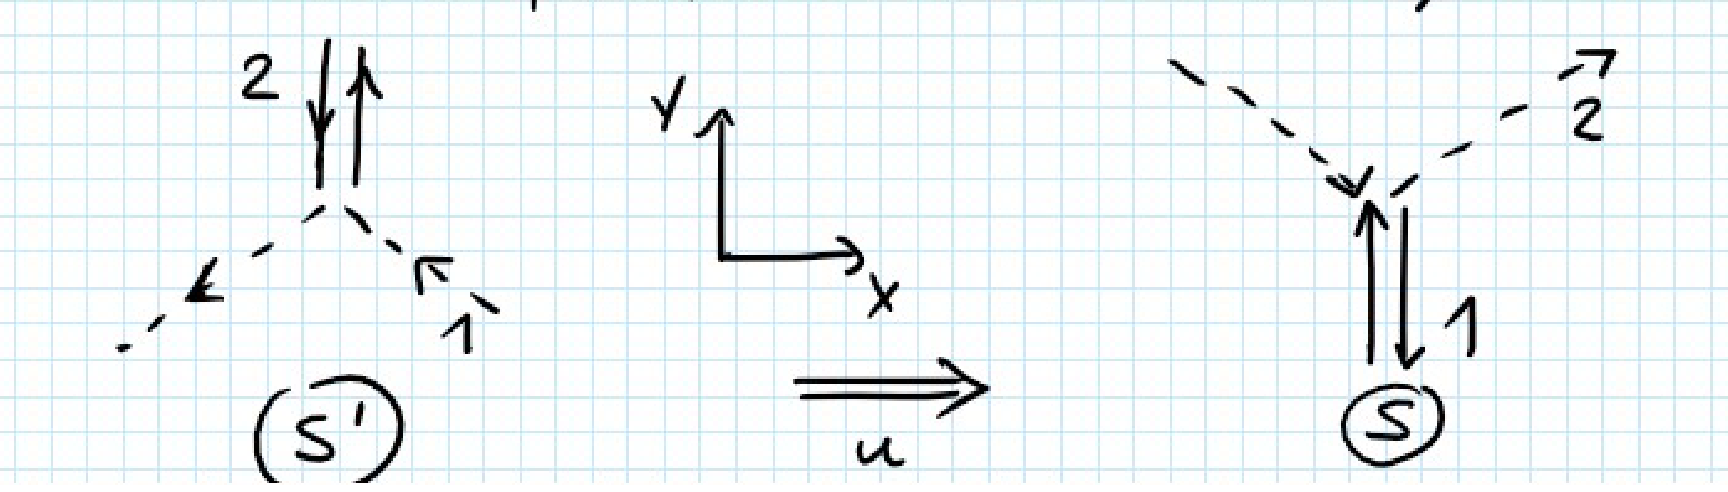
\includegraphics[width=9cm]{images/Palline_relativistiche_def_massa.png}
\end{figure}

\noindent
Considerando le formule di boost troviamo
\[\begin{cases}
(v_2)_x=\frac{0+u}{1+0}=u\\
(v_2)_y=\frac{-v_0}{\gamma(u)(1+0)}=-\frac{v_0}{\gamma(u)}.
\end{cases}\]
Imponiamo la conservazione degli impulsi (potenzialmente ammettendo che la massa dipenda dalla velocit\`a) lungo l'asse $y$:
\[2M(v_1)v_0=2M(v_2)\frac{v_0}{\gamma(u)},\]
da cui $\gamma(u)M(v_1)=M(v_2)$.\medskip

\noindent Ricordando\footnote{nota che $\vec u$ e $\vec v_1$ sono ortogonali} che $\gamma(v_2)=\gamma(v_1)\gamma(u)$ osserviamo che
\[\frac{M(v_2)}{\gamma(v_2)}=\frac{M(v_1)}{\gamma(v_1)}=\frac{M(0)}{\gamma(0)}=M(0)=m.\]

\end{example}

\begin{definition}[Massa a riposo]
Definiamo la \textbf{massa a riposo} $m$ come la massa misurata in un sistema dove il corpo \`e a riposo.
\end{definition}

\begin{definition}[Impulso relativistico]
Definiamo l'\textbf{impulso relativistico} come
\[\vec p=M(v)\vec v=m\gamma(v)\vec v.\]
\end{definition}
\begin{remark}
Con l'aumentare della velocit\`a, la ``massa effettiva" cresce molto fino a diventare ``infinita" per una velocit\`a che tende verso la velocit\`a della luce.
\end{remark}

\begin{definition}[Quadriimpulso]
Definiamo il \textbf{quadriimpulso} come
\[\wt p=m\wt v=(M(v)c,\vec p)=m\gamma(v)(c,\vec v).\]
L'impulso relativistico \`e la componente spaziale del quadriimpulso.
\end{definition}

\begin{remark}
Il modulo del quadriimpulso \`e
\[\wt p^2=m^2\wt v^2=m^2c^2.\]
In particolare il quadriimpulso \`e di tipo tempo (o di tipo luce se $m=0$).
\end{remark}

\noindent Abbiamo capito chi \`e la componente spaziale del quadriimpulso, ma la componente temporale?
\[\wt p_0c=m\gamma(v)c^2=m\gamma(v)c^2=\frac{mc^2}{\sqrt{1-\frac{v^2}{c^2}}}\]
per $v\to 0$ possiamo approssimare questa quantit\`a al primo ordine in $v^2$ come
\[mc^2-\under{\text{energia cinetica}}{\frac12 mv^2}\]

\begin{definition}[Energia]
Definiamo l'\textbf{energia} come $E=\wt p_0c$. In particolare se $v=0$ allora l'energia vale $mc^2$, che chiamiamo \textbf{energia di riposo}.
\end{definition}

\begin{remark}
L'esistenza dell'energia di riposo significa che se esiste un processo che fa diminuire la massa di un oggetto allora per conservazione dell'energia viene liberata dell'energia.\\
Questi processi esistono e vengono impiegati per l'estrazione di energia atomica.\\
Esistono processi che distruggono interamente la massa, per esempio lo scontro tra una particella e la sua antiparticella.
\end{remark}

\begin{remark}
Una volta definita l'energia possiamo riscrivere il quadriimpulso come
\[\wt p=m\wt v=(E/c,\vec p).\]
\end{remark}


\begin{remark}
Se cambiamo sistema di riferimento, l'energia cambia come segue:
\[E'=m\gamma(v')c^2=m\gamma(v)\gamma(u)(c^2-uv)=\gamma(u)(E-up_x).\]
Osserviamo che questo \`e compatibile col fatto che $\wt p$ \`e un quadrivettore, cio\`e rispetta le trasformazioni di Lorenz:
\begin{align*}
p'_x=&\frac{E' v'}{c^2}=\frac{(m\gamma(v)\gamma(u)(c^2-uv))\pa{\dfrac{v-u}{c^2-uv}c^2}}{c^2}=\\
=&m\gamma(v)\gamma(u)(v-u)=\\
=&\gamma(u)\pa{p_x-u\frac{E}{c^2}}.
\end{align*}
\end{remark}

\begin{remark}
Calcoliamo il modulo del quadriimpulso
\[m^2c^2=\wt p^2=\pa{\frac Ec}^2-(\vec p)^2,\]
cio\`e
\[\boxed{E^2=(\vec p)^2c^2+m^2c^4}\]
\end{remark}

\begin{remark}
Poich\'e $v=\frac{\abs{\vec p}c^2}E$ si ha che $\beta(v)=\frac{\abs{\vec p}c}E$ e quindi
\[\boxed{\gamma=\frac{E}{mc^2}}\]
ovvero $E=\gamma(v)mc^2$.
\end{remark}

\begin{definition}[Energia cinetica]
Definiamo l'\textbf{energia cinetica relativistica} come
\[T=E-mc^2=mc^2(\gamma(v)-1).\]
\end{definition}
\begin{remark}
Se $v$ \`e piccolo $\gamma{v}\approx 1+\frac12\frac{v^2}{c^2}$, da cui $T\approx mc^2\frac 12\frac{v^2}{c^2}=\frac12 mv^2$.
\end{remark}

\noindent Consideriamo ora questa domanda: \`e possibile che la luce sia composta da particelle?\medskip

\noindent In questo caso $\gamma(v)=\gamma(c)=\infty$, quindi affinch\'e l'energia di questa ipotetica particella abbia senso, $m=0$. In questo caso avremmo
\[E=\abs{\vec p}c.\]
Queste particelle sono dette \textbf{fotoni}.

\subsection{Terzo principio della dinamica}
Consideriamo adesso la questione delle forze uguali e contrarie. Se queste forze opposte vengono applicate allo stesso punto e allo stesso istante non abbiamo problemi.\medskip

\noindent Se le forze uguali e contrarie agiscono su punti diversi, la relativit\`a della simultaneit\`a comincia a creare problemi su \textit{quando} le due forze sono uguali e contrarie.\medskip

\noindent La soluzione \`e osservare che quello che vogliamo \`e che la variazione totale dell'impulso sia nulla. La forza deriva da variazioni di impulsi
\[\vec F_A=\dd t{\vec p_A},\quad \vec F_B=\dd t{\vec p_B},\quad \dd t{}(\vec p_A+\vec p_B)=0.\]
\bigskip

\noindent Un altro modo di interpretare la questione della simultaneit\`a \`e pensare a campi di forze piuttosto che forze generate direttamente da oggetti.

\begin{definition}[Quadriforza]
Definiamo la \textbf{quadriforza} come
\[\wt F=\dd \tau{\wt p}=m\dd\tau{\wt v}=m\wt a.\]
Una forma equivalente \`e 
\[\wt F=\dd \tau{\wt p}=\gamma(v)\pa{\frac1c\dd tE,\vec F},\]
dove $\vec F=\dd t{\vec p}$.
\end{definition}

\begin{remark}
Poich\'e $\wt v\cdot \wt a=0$ si ha che $\wt v\cdot\wt F=0$. Scrivendo esplicitamente la seconda equazione
\[\vec F\cdot \vec v=\dd tE=mc^2\dd t\gamma=m\gamma^3 \vec v\cdot \vec a.\]
\end{remark}

\begin{remark}
Troviamo le seguenti identit\`a
\[\wt F=\gamma(v)\pa{\frac{\vec F\cdot \vec v}c,\vec F}\]
\[\vec F=\dd t{\vec p}=\dd t{}(m\vec v\gamma)=m\gamma\vec a+\frac{\vec F\cdot \vec v}{c^2}\vec v,\]
in particolare \underline{$\vec F$ non \`e allineata con $\vec a$ in generale}.
\end{remark}

\begin{remark}
Osserviamo che
\[\wt F\cdot \wt v=\dd\tau{}(m\wt v)\cdot \wt v=\dd\tau m\wt v^2+m\ \under{=0}{\wt a\cdot \wt v}=c^2\dd\tau m.\]
\end{remark}

\section{Effetto Doppler}
Supponiamo che un sistema $S'$ emetta delle onde con frequenza $\nu'$ e lunghezza d'onda $\la'$ constanti (quindi i fronti d'onda hanno velocit\`a $v'=\la'\nu'$ rispetto a $S'$).

\subsection{Versione classica}
Se $S'$ si muove con velocit\`a $u$ osserviamo che
\[\la=v\Delta t'-u\Delta t'=(v-u)\Delta t'=\frac{v-u}{\nu'},\]
da cui
\[\nu=\frac v\la=\frac1{1-u/v}\nu',\]
quindi la frequenza dell'onda misurata da $S$ \`e cambiata di un fattore che dipende dalla velocit\`a relativa tra i sistemi.\medskip

\noindent Supponendo ora che sia $S$ ad emettere l'onda notiamo con calcoli analoghi che
\[\nu'=\pa{1-\frac uv}\nu,\]
che come notazione \`e la stessa di prima ma la frequenza ricevuta e quella emessa hanno scambiato i ruoli.

\subsection{Versione relativistica}
Consideriamo il caso di una sorgente in movimento $S'$ che emette l'onda (a velocit\`a $v$ in $S'$) e che si muove verso $S$.\\
Fissiamo degli eventi:
\begin{enumerate}
\item \ul{Emissione di un fronte d'onda}: In $S'$ questo evento ha coordinate $(t_e',0)$.
\item \ul{Ricezione del fronte d'onda}: In $S'$ questo evento ha coordinate $(t'_r,x'_r)$ dove $t'_r=t_e'+\delta t'$ e $x'_r=v\delta t'$. Osserviamo per\`o che $x'_r$ \`e anche l'origine di $S$ vista in $S'$. Se $x'_0$ \`e la coordinata dell'origine di $S$ al tempo $t'=0$ si ha che $x'_r=x_0'-ut_r'$.
\end{enumerate}
Mettendo tutto insieme
\[\delta t'=\frac{x'_0-ut'_e}{u+v}.\]
Consideriamo adesso due emissioni (1 e 2), una a $t_e'=0$ e $t'_e=T$. Chiaramente $\Delta t_e'=T$, mentre
\begin{align*}
\Delta t'_r=&(T+\delta t'(T)) - (0+\delta t'(0))=\\
=&T+\frac{x'_0-uT}{u+v}-\frac{x'_0}{u+v}=\\
=&T\pa{1-\frac u{u+v}}=\\
=&T\frac v{u+v}.
\end{align*}
Applichiamo adesso una trasformazione di Lorenz per passare al sistema $S$:
\[\Delta t'_r=\gamma(\Delta t_r-u\under{=0}{\Delta x_r})=\gamma \Delta t_r,\]
quindi
\[\Delta t_r=\frac T\gamma\frac v{u+v}.\]
Consideriamo ora il caso di onde luminose ($v=c$)
\[\frac1{\Delta t_r}=\nu=\nu'\gamma\frac{u+c}c=\sqrt{\frac{1+\beta(u)}{1-\beta(u)}}\nu'.\]
\bigskip

\noindent Per il principio di relativit\`a, se $S'$ si stesse allontanando e $S$ fosse la sorgente troviamo 
\[\nu'=\sqrt{\frac{1-\beta(u)}{1+\beta(u)}}\nu.\]

\bigskip

\noindent Possiamo riassumere entrambe le formule in
\[\boxed{\nu_{\mathrm{ricevuta}}=\sqrt{\frac{1+\beta}{1-\beta}}\nu_{\mathrm{emessa}}}\]



\section{Elettro-Magnetismo}
Ricordiamo la \textbf{Forza di Lorentz}
\[\vec F=q(\vec E+\vec v\times \vec B)\]

\begin{example}[Campo elettrico e campo magnetico sono la stessa cosa?]
Consideriamo un filo entro il quale scorre una corrente $I$. Vicino al filo abbiamo una carica $q<0$ che si muove a velocit\`a $v_0$ parallela al filo e in direzione opposta a $I$

\begin{figure}[!htb]
    \centering
    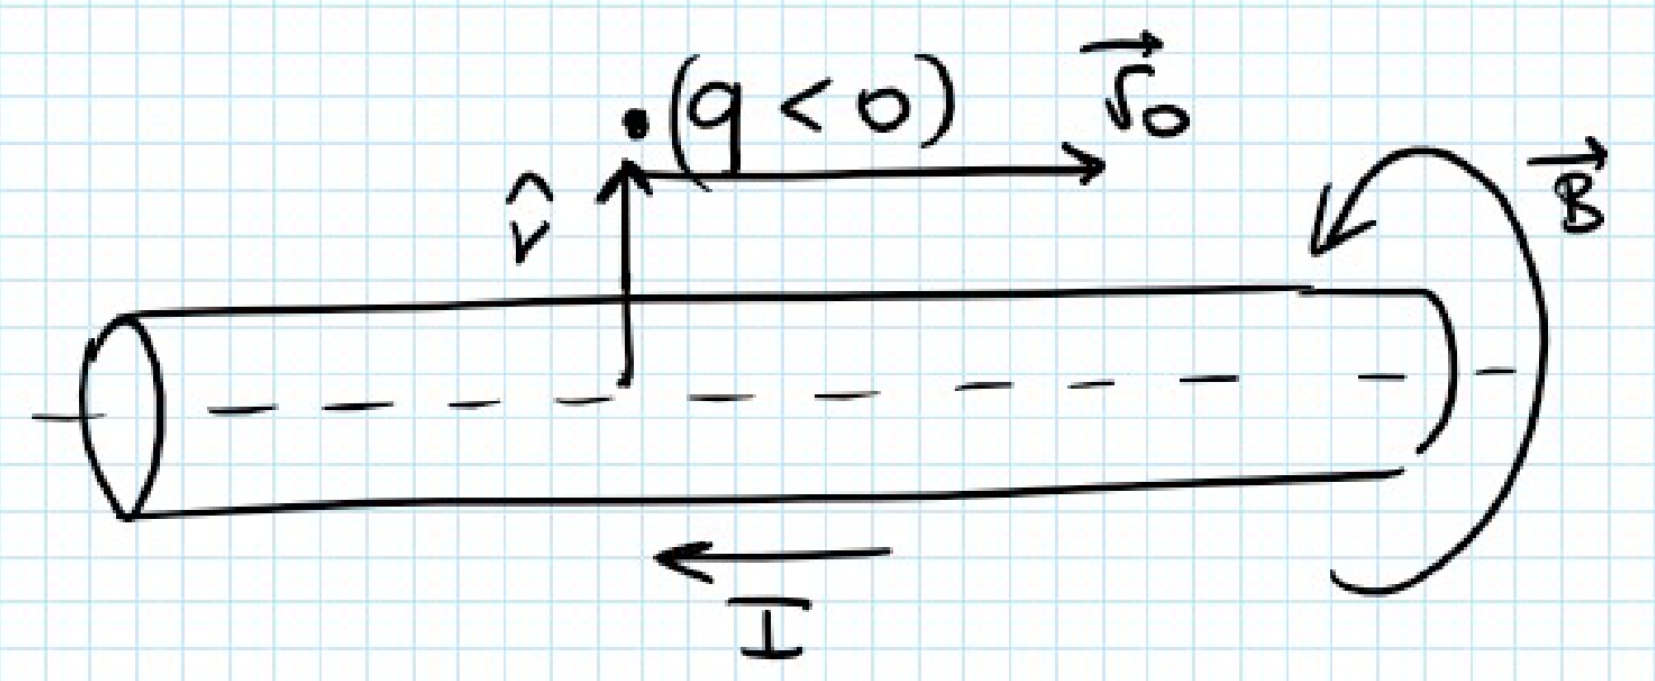
\includegraphics[width=8cm]{images/Filo_e_carica.png}
\end{figure}

\noindent
Il campo magnetico vale
\[\vec B=\frac1{4\pi \e_0c^2}\frac{2 \vec I\times \wh r}r,\]
da cui, se il filo \`e complessivamente neutro,
\[\vec F=q\vec v_0\times \vec B=\frac1{4\pi \e_0c^2}\frac{2 qIv_0}r.\]
Mettiamoci ora in un sistema dove $q$ ha velocit\`a nulla. Abbiamo una forza di Lorentz?
\medskip

\noindent Si verifica sperimentalmente che $q$ \`e invariante per trasformazioni di Lorentz. Quindi se $\vec v'=0$ l'unica speranza \`e $\vec E$.\\
Poich\'e le distanze cambiano sotto una trasformazione di Lorenz, \`e ragionevole pensare che la densit\`a di carica cambi: 

\begin{figure}[!htb]
    \centering
    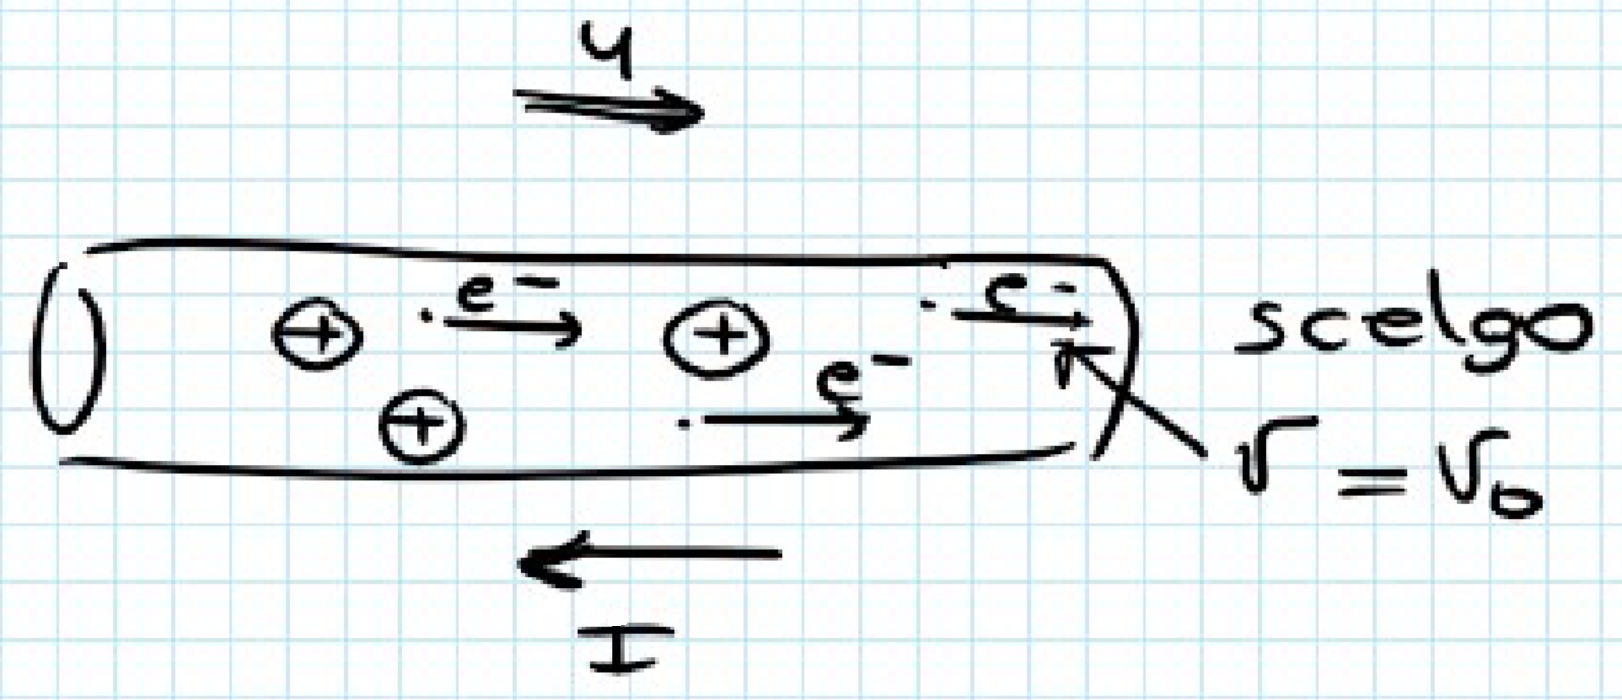
\includegraphics[width=8cm]{images/corrente_in_filo.png}
\end{figure}

\noindent
Se $L$ \`e la lunghezza di un pezzo del filo e $A$ \`e l'area di una sezione del filo,
\[\rho=\frac q{LA}\leadsto \rho'=\frac q{L'A}=\gamma \rho.\]
Nel sistema $S'$ la densit\`a delle cariche positive \`e $\rho'_+=\rho_+\gamma$. Considerando ora le cariche negative (che si spostano per trasportare la corrente a velocit\`a $v$ in verso opporto a $I$), per semplicit\`a scegliamo $I$ tale che $v=v_0$ \`e la velocit\`a della particella, vediamo che con questa scelta in $S'$ queste cariche sono ferme, quindi $\rho_-=\gamma \rho_-'$. Poich\'e avevamo supposto che il filo fosse neutro in $S$ si ha che $\rho_+=-\rho_-$, quindi \[\rho_+'=\rho_+\gamma=-\rho_-\gamma=-\gamma^2\rho_-',\]
in particolare $\rho_+'\neq \rho_-'$ quindi il filo non \`e pi\`u neutro! Pi\`u precisamente
\[\rho'=\rho'_++\rho_-'=\rho_+\pa{\gamma-\frac1\gamma}>0\]
Il campo elettrico generato ha modulo
\[E'=\frac{\rho' A}{2\pi\e_0r}=\frac{\rho_+A\frac{v^2}{c^2}}{2\pi\e_0 r\sqrt{1-v^2/c^2}},\]
dunque c'\`e una forza di Lorentz pari a 
\[F'=q\frac{\rho_+A\frac{v^2}{c^2}}{2\pi\e_0 r\sqrt{1-v^2/c^2}}.\]
Confrontiamo questa forza con quella trovata prima:
\[F=\frac1{4\pi \e_0c^2}\frac{2 qIv_0}r\pasgnlmath={I=\rho_-Av}q\frac{-\rho_- Av \frac{v_0}{c^2}}{2\pi \e_0 r}\pasgnlmath={v=v_0}q\frac{\rho_+ A \frac{v^2}{c^2}}{2\pi \e_0 r}\]
che \`e esattamente $F'/\gamma$ come speravamo.
\end{example}

\begin{definition}[Quadrivettore densit\`a di corrente]
Definiamo la \textbf{densit\`a di carica propria} come la densit\`a di carica misurata in un sistema dove l'oggetto \`e fermo.\\
Se $\rho_0$ \`e la densit\`a di carica propria allora in un sistema dove l'oggetto si muove a velocit\`a $v$ la densit\`a di carica \`e
\[\rho=\rho_0\gamma(v).\]
Definiamo la \textbf{densit\`a di corrente relativistica} come
\[\vec J=\rho\vec v=\rho_0\gamma(v)\vec v.\]
Definiamo la \textbf{quadricorrente} come
\[\wt J=(\rho c,\vec J)=\rho_0\gamma(v)(c,\vec v)=\rho_0\wt v.\]
\end{definition}


\begin{remark}[Teorema di Gauss relativistico]
Calcoliamo
\[\wt \nabla \cdot \wt J=\frac1c\pp t{(\rho c)}+\pp x{J_x}+\pp y{J_y}+\pp z{J_z}=\pp t\rho+\vec\nabla \cdot \vec J=0\]
dove l'ultima uguaglianza \`e la legge di continuit\`a\footnote{cio\`e la conservazione della carica.}. Quindi possiamo effettivamente riscrivere la conservazione della carica come
\[\wt\nabla\cdot \wt J=0\]
e questa formulazione \`e evidentemente compatibile con la relativit\`a.
\end{remark}

\noindent
Ricordiamo che $\phi$ e $\vec A$ sono definiti in modo tale che
\[\begin{cases}
\vec E=-\pp t{\vec A}-\vec \nabla \phi\\
\vec B=\vec \nabla \times \vec A
\end{cases}\]

\begin{definition}[Quadripotenziale]
Definiamo il \textbf{quadripotenziale} come
\[\wt A=(\phi/c,\vec A).\]
\end{definition}


\begin{remark}
Le equazioni di Maxwell si possono riscrivere come
\[\begin{cases}
\square\phi=\rho/\e_0\\
\square \vec A=\mu_0\vec J
\end{cases}\]
quindi una forma compatta per le equazioni di Maxwell \`e
\[\square\wt A=\mu_0\wt J,\]
che mostra immediatamente che sono compatibili con la relativit\`a.
\end{remark}
\begin{proof}
Le equazioni di Maxwell sono
\[\begin{cases}
\vec\nabla\cdot \vec E=\frac\rho{\e_0},\\
\vec\nabla\cdot\vec B=0,\\
\vec \nabla \times \vec E=-\pp t{\vec B},\\
\vec \nabla \times \vec B=\mu_0\pa{\vec J+\e_0\pp t{\vec E}}
\end{cases}\]
Sostituendo le espressioni per $\vec E$ e $\vec B$ in termini di $\phi$ e $\vec A$ troviamo
\[\begin{cases}
\pp t{}\vec\nabla\cdot \vec A +\nabla^2 \phi=-\frac\rho{\e_0},\\
\vec \nabla \times (\vec \nabla \times \vec A)=\mu_0\pa{\vec J-\e_0\pps[2] t{\vec A}-\e_0\pp t{}\vec \nabla \phi}=\mu_0\vec J-\frac1{c^2}\pps[2]t{\vec A}-\frac1c\pp t{}\vec\nabla(\phi/c)
\end{cases}\]
\[\begin{cases}
-\nabla^2 \phi=\frac\rho{\e_0}+\pp t{}\vec\nabla\cdot \vec A,\\
-\nabla^2\vec A+\vec\nabla(\vec\nabla\cdot\vec A)=\mu_0\vec J-\frac1{c^2}\pps[2]t{\vec A}-\frac1c\pp t{}\vec\nabla(\phi/c)
\end{cases}\]
\[\begin{cases}
\square \phi = \frac\rho{\e_0}+\pp t{}\pa{\wt \nabla \cdot \wt A},\\
\square\vec A +\vec\nabla(\vec\nabla\cdot\vec A)=\mu_0\vec J-\frac1c\pp t{}\vec\nabla(\phi/c)
\end{cases}\]
\[\begin{cases}
\square \phi =\frac\rho{\e_0}+\pp t{}\pa{\wt \nabla \cdot \wt A},\\
\square\vec A =\mu_0\vec J-\vec\nabla\pa{\wt \nabla \cdot \wt A}  
\end{cases}\]
Uniamo ora le due equazioni dividendo la prima per $c$ e poi sommando
\[\square \wt A=\mu_0\wt J +\wt \nabla(\wt \nabla\cdot \wt A),\]
per concludere possiamo scegliere il Gauge $\wt \nabla \cdot \wt A=0$.
\end{proof}

\noindent
Se definiamo $A^0=\phi/c$, notiamo che
\[\pp z{A^0}-\pp{ct}{A_z}=\frac1c\pa{\pp z\phi-\pp t{A_z}},\]
che sembra la componente $z$ di $\vec E$ divisa per $c$, ma non tornano i segni. Osserviamo per\`o che
\[\frac{E_z}c=-\pp z{\phi/c}-\frac1c\pp t{A_z}=\pa{-\pp z{}}A^0-\pa{\frac1c\pp t{}}A_z.\]
Ispirandoci a questo tipo di equazioni definiamo
\begin{definition}[Tensore elettromagnetico]
Definiamo il \textbf{tensore elettromagnetico} come
\[F_{\mu\nu}=\wt \nabla_\mu\wt A_\nu-\wt \nabla_\nu\wt A_{\mu},\]
o in forma matriciale
\[F_{\mu\nu}=\mat{
0 & E_x/c & E_y/c & E_z/c\\
-E_x/c & 0 & -B_z& B_y\\
-E_y/c & B_z& 0  & -B_x\\
-E_z/c &-B_y& B_x& 0  \\
}\]
\end{definition}

\noindent
Cerchiamo di capire come si trasforma: Se $\vec u$ \`e parallelo all'asse $x$,
\[\begin{cases}
E_x'=E_x\\
E'_y=\gamma(E_y-u B_z)\\
E'_z=\gamma(E_z-u B_y)\\
B'_x=B_x\\
B'_y=\gamma(B_y-u/c^2 E_z)\\
B'_z=\gamma(B_z+u/c^2 E_y)
\end{cases}\]
Le equazioni di Maxwell diventano
\[\sum_\mu\wt \nabla_\mu F^{\mu\nu}=\mu_0 \wt J^\nu.\]